\documentclass{article}
\usepackage[utf8]{inputenc}
\usepackage[english]{babel}

\textwidth 16.2cm \textheight 21cm \topmargin -0.6cm
\oddsidemargin 0.31cm \evensidemargin -0.91cm

\usepackage{amsmath}
\usepackage{amsfonts}
\usepackage{amsbsy}
\usepackage{amssymb}
\usepackage{algorithm2e}
\usepackage{graphicx}
\usepackage{psfrag}
\usepackage{epsfig}
\usepackage{multicol}
\usepackage{cite}
\usepackage{color}
\usepackage{dsfont}
\usepackage[center]{caption}
\usepackage{listings} 
\usepackage{xcolor} 
\usepackage{textcomp} 
%\usepackage{enumitem}

\newcommand {\defeq}    {\stackrel{\rm def}{=}}

\DeclareMathOperator{\Span} {{Span}}
\DeclareMathOperator{\gap} {{gap}}
\DeclareMathOperator{\ddiv} {{div}}
\DeclareMathOperator{\argsup} {{argsup}}
\DeclareMathOperator{\argmin} {{argmin}}
\DeclareMathOperator{\dom} {{dom}}
\DeclareMathOperator{\epi} {{epi}}

\newtheorem{thm}{Theorem}
\newtheorem{prop}{Proposition}
\newtheorem{lemma}{Lemma}
\newtheorem{defn}{Definition}
\newtheorem{cor}{Corollary}
\newtheorem{model}{Model}
\newtheorem{rmk}{Remarque}
\newtheorem{ans}{Answer}
\newtheorem{ass}{Assumption}
\newtheorem{algo}{Algorithme}

\def\endproof{\hfill $\Box$\newline\newline}
\def\proof{\par\noindent{\it Proof}. \ignorespaces}

\newcommand{\I}{\textbf{I}}
\newcommand{\B}{\textbf{B}}
\newcommand{\N}{\textbf{N}}
\newcommand{\Nd}{\textbf{N$_d$}}
\newcommand{\kernel}{\textbf{k}}
\newcommand{\ksize}{\textbf{k$_{size}$}}
\newcommand{\Isize}{\textbf{n}}

\title{Image Deblurring with Blurred/Noisy Image Pairs}
\author{Yohann Salaun}
\date{\today}

\parindent=0pt
\begin{document}
\maketitle

\section*{Introduction}

Taking a picture under low light condition often results in bad quality images. With SLR cameras, options as ISO, exposure time and aperture can be better chosen to fit the bad light conditions. However, even with such gears, the picture is not perfect when taken with hands only. A noise/blur dilemma appears and it is often impossible to avoid at least one of these artifacts. The aim of \cite{deblur_denoise} is to mix up two pictures facing a strong noise for one and a strong blur for the other in order to create a picture that is nor noisy nor blurry.


\begin{figure}[ht]
\begin{center}
	\begin{tabular}{c}	
		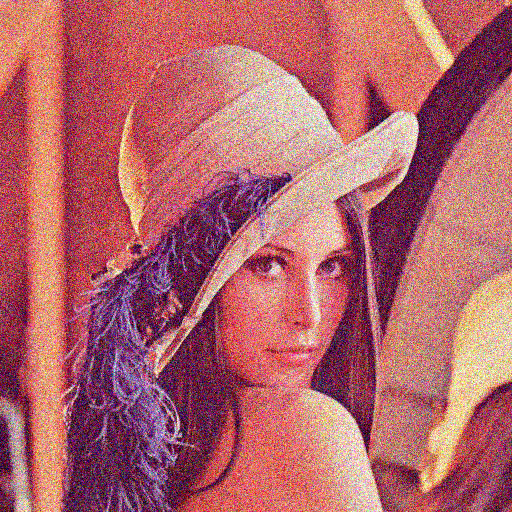
\includegraphics[scale=0.28]{images/lena_noisy.jpg}
		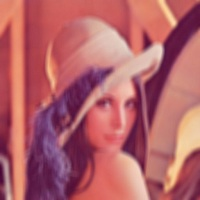
\includegraphics[scale=0.28]{images/lena_blurred.jpg}
		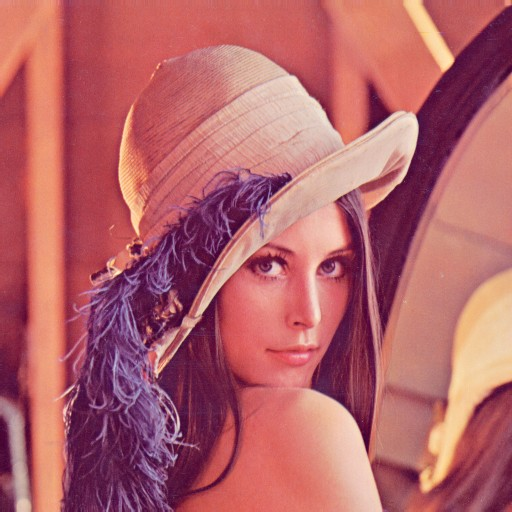
\includegraphics[scale=0.28]{images/lena.jpg}
	\end{tabular}
	\caption{On the left, the noisy picture and on the center the blurry one. Both of these pictures have been virtually altered from the left one.}
	\label{intro}
\end{center}
\end{figure}

The original article \cite{deblur_denoise} proposes a complex method that uses deblurring and denoising to improve image quality. In this report only a part of their method will be exposed and implemented.\\
In order to have a comparison for the denoising, the deblurring and the estimated kernel, the images used as input will be virtually noised/blurred versions of a picture.

\newpage

\section{Algorithm Overview}

The general idea of this algorithm is to use the noisy picture in order to find a good estimate of the blur kernel and then use it to deconvolve the blurry picture.\\

\begin{algorithm}[H]

\textbf{Input} : Noisy picture \N, Blurry picture \B, estimated kernel size \ksize\\
\textbf{Output} : Estimated picture \I, estimated kernel \kernel \\
	\Nd = denoise(\N)\\ 
	\I  = \Nd  \\
	\While{ change $> \epsilon$}{
		\textbf{Estimate} kernel \kernel\ with \I\ and \B\ s.t. \B\ = \I\ $\otimes$ \kernel.\\
		\textbf{Deconvolute} blurred picture \B.\\
		\textbf{Mix} informations to improve estimation \I.\\
		\textbf{Compute} \textit{change} between 2 iterations.
	}
\caption{Main algorithm}

\end{algorithm}

\section{ Theoretical Description }

In this section, \I\ will refer to the current estimate of the good quality picture, \B\ will be the blurry input picture and \N\ the roughly denoised version of the noisy input picture.

\subsection{ Initialization }

When taken with cameras, \N\ and \B\ have different color intensities for their pixels even when the noise and the blur does not affect them. This is due to the difference in the camera settings when the pictures are taken. In order to have the same intensity scale, \N\ is pre-multiplied by a ratio $\frac{ISO_{\B} \Delta t_{\B}}{ISO_{\N} \Delta t_{\N}}$ where $\Delta t$ is the exposure time.\\
As I used images with virtual blur/noise, I skipped this step of intensity scaling.\\

\begin{figure}[ht]
\begin{center}
	\begin{tabular}{c}	
		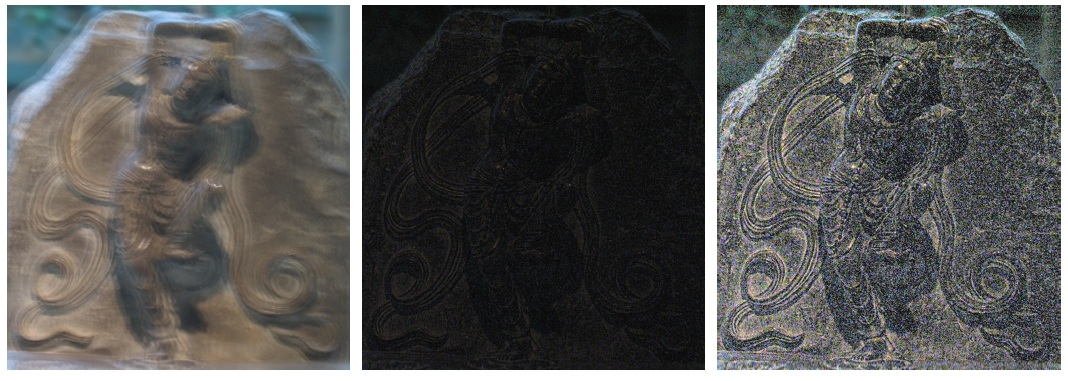
\includegraphics[scale=0.5]{images/enhanced.jpg}
	\end{tabular}
	\caption{On the left, the blurry picture and on the center the noisy one. The left one is the noisy picture multiplied by the exposure ratio in order to have comparable intensity measures between the blurry and noisy pictures.}
	\label{enhanced}
\end{center}
\end{figure}

\newpage

Then the noisy picture \N\ is denoised by an extern process. \cite{deblur_denoise} proposes to use the wavelet based algorithm developed by \cite{rough_denoise}.\\
However, as this code is no more available, I used a simple bilateral filter to roughly denoise \N\ into $\Nd$. The denoised picture is used to initialize the estimated picture \I.

\begin{figure}[ht]
\begin{center}
	\begin{tabular}{c}	
		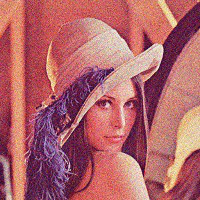
\includegraphics[scale=0.35]{images/noisy.png}
		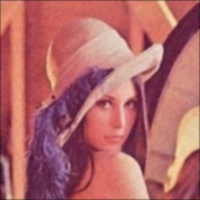
\includegraphics[scale=0.35]{images/denoised.png}
	\end{tabular}
	\caption{On the left, the noisy picture and on the right the denoised picture obtained with a simple bilateral filter.}
	\label{noisy}
\end{center}
\end{figure}

\subsection{ Kernel Estimation }

The aim of this part is to estimate the blur kernel that transformed \I\ into \B. The method exposed in \cite{deblur_denoise} is based on a gradient descent.\\ 
The problem is thus formulated as the finding the solution of:
\begin{equation}
	\B = \I\kernel
\label{kernel_eq}
\end{equation}
where $\kernel \in \mathbb{R}^{\ksize}$ and $\B \in \mathbb{R}^{\Isize}$ are written into column-vector form and $\I  \in \mathbb{R}^{\Isize \times \ksize}$ is such that $\B = \I \otimes \kernel$.\\
Solving \eqref{kernel_eq} can be done in a least square sense and the Tikhonov regularization method has been adopted in \cite{deblur_denoise}:

\begin{equation}
\min_{\kernel \in \mathbb{R}^{\ksize}} ||\I\kernel - \B||_2^2 + \lambda^2||\kernel||_2^2, \ \ s.t. \ \ \kernel \in \mathbb{R}^{+\ksize} \ \ and \ \ ||\kernel||_1 = 1 
\label{kernel_eq2}
\end{equation}

To find the minimum of \eqref{kernel_eq}, a method similar to projected gradient descent is applied:
\begin{itemize}
	\item[$\bullet$] $\kernel^0$ is initialized as the delta function.
	\item[$\bullet$] $\kernel^{n+1} = \kernel^n + \tau\nabla F(\kernel^n) = \kernel^n + 2\tau(\I^T\B - (\I^T\I +\lambda^2Id)\kernel^n)$
	\item[$\bullet$] $\kernel^{n+1} = Proj_K(\kernel^{n+1})$
\end{itemize}

where $F$ is the functional minimized in \eqref{kernel_eq}, $\tau$ the step and $K=\{\kernel \in \mathbb{R}^{+\ksize} s.t. ||\kernel||_1 = 1 \}$. \\
In \cite{deblur_denoise}, the projection on $K$ is build this way:

\begin{itemize}
	\item[$\bullet$] positive the kernel coefficients $\kernel_i= max(\kernel_i, 0)$
	\item[$\bullet$] normalize the kernel $\kernel = \frac{\kernel}{||\kernel||}$
\end{itemize}

This method is a bit questionable since it is not a real projection and some points are projected on the null kernel.\\
\\
After some unsuccessful try with this algorithm, I finally used the gradient descent algorithm without projection and used a projection at the end only in order to have a correct blur kernel.

\subsection{Deconvolution}

Once the blur kernel has been estimated, it can be used in order to find a better estimate of the final picture. The deconvolution is then performed with the standard Richardson-Lucy algorithm.\\
This method is an iterative one that needs the blurred picture \B, the estimated kernel \kernel\ and an initialization of the picture which here will be \I.\\
The standard form of the algorithm uses the iterative formula:
\[
	\I^{k+1} _i= \I^k_i \sum_{j}\frac{\B_j}{(\kernel \otimes \I^k)_j} \kernel_j[i]
\]
where $\kernel_j[i]$ is the $j^{th}$ coefficients of the kernel \kernel\ centered in pixel $i$.\\

In order to have better results for the deconvolution, \cite{deblur_denoise} propose to use the residual pictures :
\begin{itemize}
	\item[$\bullet$] $\Delta \I = \I - \Nd$
	\item[$\bullet$] $\Delta \B = \Delta \I \otimes \kernel = \B - \Nd \otimes \kernel$
\end{itemize}

The idea that motivates this change is that the RL-deconvolution often creates a ringing effect around the picture and the ringing effect of residual pictures will be at their scale, which is small compared to the whole pictures.\\
An offset is also added to each residual in order to avoid zero value for color intensities. The offset value is 1 when the color intensities are normalized to range [0, 1].\\
\\
When I tested the algorithm on the pictures in FIG.\ref{intro}, the deconvolution worked well for the whole pictures but the residual one had really bad results. Thus I could not really apply this part with my own pictures.

\subsection{De-ringing}

The aim of this part is to avoid the ringing effect and mix the pictures in order to have sharp details in the final picture.\\
The ringing effect is a consequence of the Gibbs phenomena in Fourier analysis and appear near border. Since, its effect are stronger when the kernel size is larger, it can be an important artifact in the output of such a method. Moreover, as the blur kernel is an unknown parameter, the larger its estimated size is, the better the kernel estimation can be done. Thus, decreasing the ringing effect will allow better estimations of the optimal picture.\\
In order to avoid ringing effects, the algorithm used is a slight variation of the RL-deconvolution :

\[
	\I^{k+1} _i= I_{GAIN}[i](\I^k_i \sum_{j}\frac{\B_j}{(\kernel \otimes \I^k)_j} \kernel_j[i])
\]

$I_{GAIN}[i]$ is a multiplier factor that is here to decrease the contrast of the residual pictures since the ratio $\sum_{j}\frac{\B_j}{(\kernel \otimes \I^k)_j} \kernel_j[i]$ increase its magnitude at each iteration.\\
\\
The gain map $I_{GAIN}$ is computed in order to be lower in flat region (i.e. where the ringing effect appears) and higher in edges regions :

\[
	I_{GAIN} = 	(1 - \alpha) + \alpha \sum_l \| \nabla \Nd^l \|
\]

The authors of \cite{deblur_denoise} are not very explicit about the computation of this gain map. Moreover, as I only manipulated small pictures and small kernels (due to computation time) I did not really observed the ringing effect. Thus I did not implemented this part of the algorithm.\\
\\
The algorithm results are now a picture \I\ with details and ringing effects obtained from residual RL and the "opposite" picture $\I_g$ with bad details but no ringing effect. The idea is then to mix these two pictures in order to have an estimate \I\ that has nor ringing effects, nor bad details.\\
The method used is highly inspired from HDR algorithm :

\begin{itemize}
	\item[$\bullet$] Compute a detail layer $\I_d = I - F(I)$ where $F$ is a low-pass filter such as the bilateral filter
	\item[$\bullet$] Compose the detail layer $\I_d$ and the base layer $\I_g$
\end{itemize}

Once again, as I did not observed the ringing effects, I could not implemented this part of the algorithm.

\section{Results}

Since the computation has been very slow, I used only small resolution pictures (200 x 200 pixels) and small kernels ($5\times5$ pixels or $9\times9$ pixels). \\
The original pictures, the estimations and the kernel estimations can be seen in FIG. \ref{lena_5px} and FIG. \ref{lena_9px}. \\

\begin{figure}
\begin{center}
	\begin{tabular}{c}	
		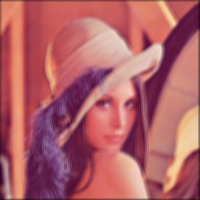
\includegraphics[scale=1]{images/blurred_5px.png}
		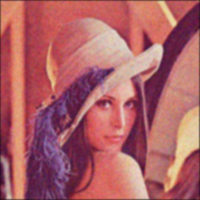
\includegraphics[scale=1]{images/denoised_5px.png}\\
		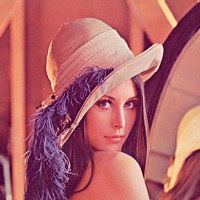
\includegraphics[scale=1]{images/original_5px.png}
		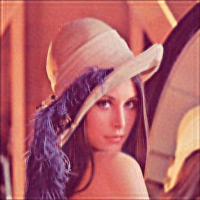
\includegraphics[scale=1]{images/estimation_5px.png}\\
		
\includegraphics[scale=1]{images/kernels_5px.png}
	\end{tabular}
	\caption{On the top left, the blurred picture obtained with a $5\times5$ kernel and on top the right the denoised picture obtained with a simple bilateral filter. The bottom left is the original picture and the right one is the estimation obtained with the algorithm. The last picture is a comparison between the original blur kernel on the left and its estimation on the right.}
	\label{lena_5px}
\end{center}
\end{figure}

\begin{figure}
\begin{center}
	\begin{tabular}{c}	
		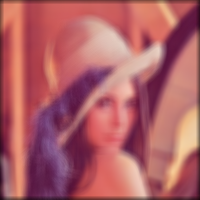
\includegraphics[scale=1]{images/blurred_9px.png}
		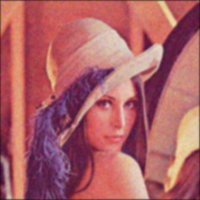
\includegraphics[scale=1]{images/denoised_9px.png}\\
		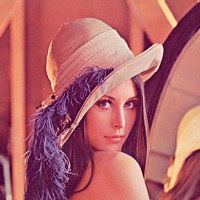
\includegraphics[scale=1]{images/original_5px.png}
		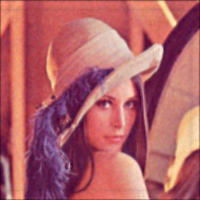
\includegraphics[scale=1]{images/estimation_9px.png}\\
		
\includegraphics[scale=0.7]{images/kernels_9px.png}
	\end{tabular}
	\caption{On the top left, the blurred picture obtained with a $9\times9$ kernel and on top the right the denoised picture obtained with a simple bilateral filter. The bottom left is the original picture and the right one is the estimation obtained with the algorithm.The last picture is a comparison between the original blur kernel on the left and its estimation on the right.}
	\label{lena_9px}
\end{center}
\end{figure}

\begin{figure}
\begin{center}
	\begin{tabular}{c}	
		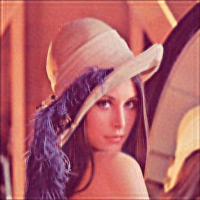
\includegraphics[scale=1]{images/estimation_5px.png}
		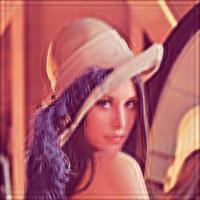
\includegraphics[scale=1]{images/estimation_0.png}
		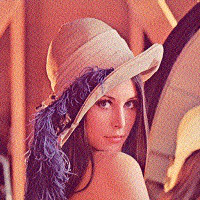
\includegraphics[scale=1]{images/estimation_N.png}\\
		
\includegraphics[scale=1]{images/kernels_5px.png}
		
\includegraphics[scale=1]{images/kernels_0.png}
		
\includegraphics[scale=1]{images/kernels_N.png}
	\end{tabular}
	\caption{Comparison of results obtained with different initialization for \I. From left to right, $\I^0 = \Nd,\ \I^0 = 0,\ \I^0 = \N$ }
	\label{init}
\end{center}
\end{figure}

\begin{figure}
\begin{center}
	\begin{tabular}{c}
		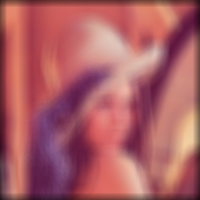
\includegraphics[scale=1]{images/blurred_15_5.png}
		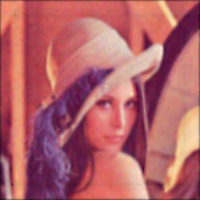
\includegraphics[scale=1]{images/estimation_15_5.png}\\
		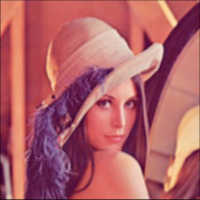
\includegraphics[scale=1]{images/blurred_3_9.png}
		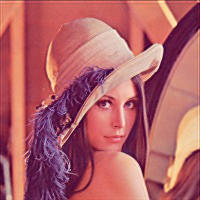
\includegraphics[scale=1]{images/estimation_3_9.png}
	\end{tabular}
	\caption{Leftward pictures are blurry inputs and rightward ones are estimations. Comparison of results obtained with differences between real kernel size and estimated kernel size. Up pictures are obtained with a real kernel size of 15 pixels and an estimated one of 5 pixels. Bottom pictures are obtained with a real kernel size of 3 pixels and an estimated one of 9 pixels. }
	\label{kernel_size}
\end{center}
\end{figure}


As we can see, the estimated kernel is very influenced by its Dirac initialization. However, lowering the $\lambda$ coefficient in \eqref{kernel_eq2} does not change a lot the result.\\

FIG. \ref{init} illustrates the results difference obtained with different initialization :

\begin{itemize}
	\item[$\bullet$] $\I^0 = 0$ obtains similar result to the classical method for the kernel estimation. However, the ringing artifact supposed to appear with classical method can be seen.
	\item[$\bullet$] $\I^0 = \N$ obtains better estimation for the blur kernel but keeps a lot of noise in the final estimation.
\end{itemize}

This observation seems to confirm that using the noisy picture to estimate the blur kernel is a good idea but maybe denoising it at the early beginning is too soon for a good information on the blur kernel.

\newpage

\section{Conclusion}

The results I obtained with my algorithm cannot really be compared with the results obtained in \cite{deblur_denoise} because only a part of it was really implemented and due to computation time, I used only small scales instead of more realistic one (8 Mpixels pictures and 64 $\times$ 64 kernels).\\
In fact, the kernel size is a very important parameter because, as the real blur kernel is unknown, the larger the estimation is, the better the results should be. If the estimated blur kernel is bigger than the real one, the estimation is far better than in the opposite case (see FIG.\ref{kernel_size}). \\
Moreover, the cases I used were virtual pictures while for real pictures, the blur in \B\ is caused by the long exposure time but also by the camera movement between the first shoot \N\ and the second one \B.\\
Finally, I think that mixing informations coming from a blurry picture and a noisy picture if the same scene is a great idea and \cite{deblur_denoise} seems to show that it works greatly. However, this article is always very explicit and I could not implement and observe all of what they did.

\begin{thebibliography}{9}

\bibitem{rough_denoise}
	J. Portilla, V. Strela, M. Wainwright, and E.P. Simoncelli
	\emph{Image denoising using scale mixtures of gaussians in the wavelet domain}.
	IEEE
	Trans. on Image Processing 12, 11, 1338–1351,
	2003.

\bibitem{deblur_R}
	H. Richardson
	\emph{ Bayesian-based iterative method of image restoration}.
	JOSA, A 62, 1, 55–59.
	1972.

\bibitem{deblur_denoise}
	L. Yuan, J. Sun, L. Quan, and H-Y. Shum
	\emph{Image Deblurring with Blurred/Noisy Image Pairs}.
	ACM SIGGRAPH,
	2007. 

\end{thebibliography}


\end{document}
